\section{Structural Similarity Index Measure}

Structural Similarity Index Measure (SSIM) \cite{wang2004image} is a metric used to calculate the similarity between two images. It measures a perceived change in the structural information between images and is used for picture comparison in television. The index does not use the whole image but rather $NxN$ windows to calculate similarity scores. The window size used in the original paper is $11x11$, and if not specified otherwise, this is a window used in my work. The SSIM is defined as:

\begin{equation}
    {\displaystyle {\hbox{SSIM}}(x,y)={\frac {(2\mu _{x}\mu _{y}+(k_1L)^2)(2\sigma _{xy}+(k_2L)^2)}{(\mu _{x}^{2}+\mu _{y}^{2}+(k_1L)^2)(\sigma _{x}^{2}+\sigma _{y}^{2}+(k_2L)^2)}}}
    \label{eq:ssim}
\end{equation}

Where $x$ and $y$ are the images to compare, $mu _{x}$ and $mu _{y}$ are the mean values of pixels from the window. $\sigma _{x}$ and $\sigma _{y}$ are the variance of those pixels from the window, and $\sigma _{xy}$ is a covariance of $x$ and $y$. There is also the $L$ parameter, which is important when trying to compare SSIM values calculated for the images from different distributions. This parameter defined a dynamic range of values present in the image. In the case of comparing attributions, it usually is a maximum value of attribution from a given dataset (assuming the same attribution method and model). Values of $k_1$ and $k_2$ are constant and equal to $0.01$ and $0.03$ accordingly.

\begin{figure}[h]
  \centering
 \begin{subfigure}{.3\textwidth}
    \centering
    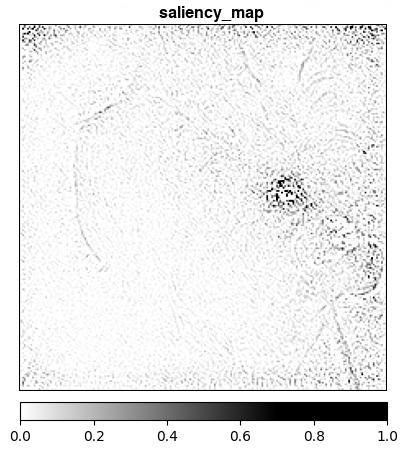
\includegraphics[width=\textwidth]{methods/images/cairn-none.jpg}
    \caption{Baseline}\label{fig:ssim-carin-none}
\end{subfigure}
 \begin{subfigure}{.3\textwidth}
    \centering
    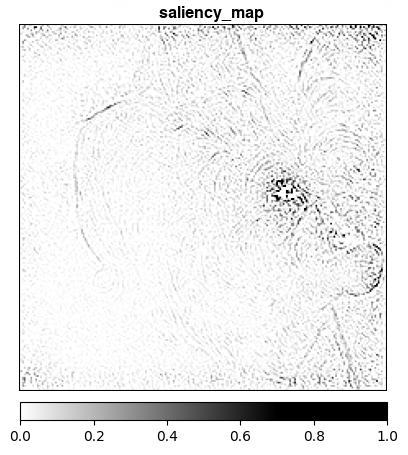
\includegraphics[width=\textwidth]{methods/images/cairn-sharp.jpg}
    \caption{$SSIM = 0.955$}\label{fig:ssim-carin-sharp}
\end{subfigure}
 \begin{subfigure}{.3\textwidth}
    \centering
    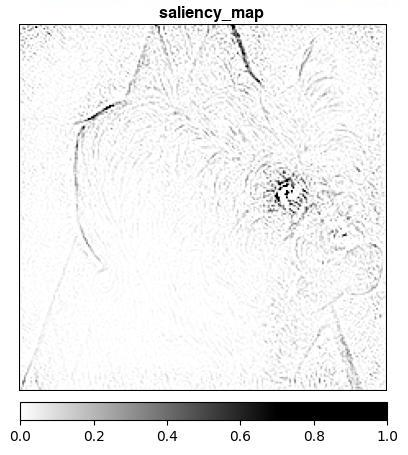
\includegraphics[width=\textwidth]{methods/images/cairn-norm.jpg}
    \caption{$SSIM = 0.885$}\label{fig:ssim-carin-norm}
\end{subfigure}

 \caption{SSIM scores for comparing the baseline attribution (Fig. \ref{fig:ssim-carin-none}) with attributions of augmented images. Image source: \textit{Stanford Dogs} \cite{stanford-dogs} }\label{fig:ssim-scores-example}
\end{figure}

The amount SSIM value change with the change in the perception of the image is presented in Figure \ref{fig:ssim-scores-example}. The higher score achieved when comparing image \ref{fig:ssim-carin-none} with \ref{fig:ssim-carin-sharp} can be related to the visual similarity between two images. We can clearly see that attribution from image \ref{fig:ssim-carin-norm} is sharper, and therefore less similar to the baseline.

\begin{remark}
Quantifying human visual perception is still an active field of research, and SSIM metric is not the perfect solution. There are other methods, but they all had some issues when compared with real humans. This metric is going to be used to qualitatively compare attributions because comparing thousands of images qualitatively is not possible in a reasonable amount of time.
\end{remark}